\documentclass[border=1pt]{standalone}
\usepackage[T1]{fontenc}
\usepackage{mathptmx}
\usepackage{amsmath}
\usepackage{xcolor}
\usepackage{pgfplots}
\usepackage{pgfplotstable}
\pgfplotsset{compat=1.17}
\usepgfplotslibrary{groupplots}
\usetikzlibrary{positioning,calc}
\definecolor{cStd}{RGB}{0,114,178}
\definecolor{cRFM}{RGB}{230,159,0}
\definecolor{cCon}{RGB}{0,158,115}
\definecolor{cML}{RGB}{213,94,0}
\definecolor{cCL}{RGB}{86,180,233}
\definecolor{aHigh}{RGB}{213,94,0}
\definecolor{aReg}{RGB}{0,114,178}
\definecolor{aOcc}{RGB}{0,158,115}
\definecolor{aLap}{RGB}{160,160,160}
\begin{document}
\setlength{\columnwidth}{252pt}\setlength{\textwidth}{516pt}
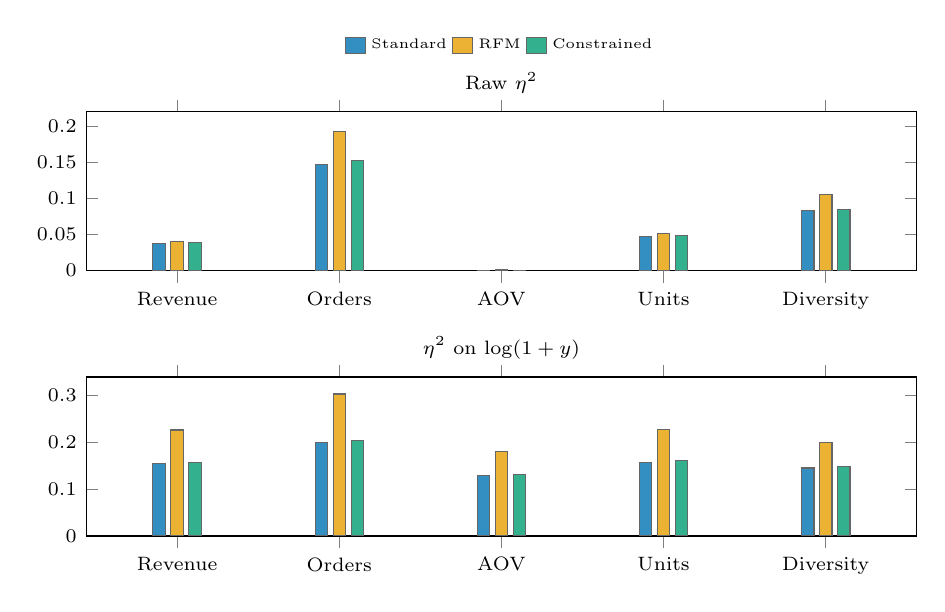
\begin{tikzpicture}
\begin{groupplot}[
  group style={group size=1 by 2, vertical sep=1.35cm},
  width=\columnwidth, height=3.6cm,
  ybar, /pgf/bar width=4.5pt,
  symbolic x coords={Rev,Ord,AOV,Units,Div}, xtick=data,
  xticklabels={Revenue,Orders,AOV,Units,Diversity},
  x tick label style={font=\scriptsize},
  y tick label style={font=\scriptsize, /pgf/number format/fixed},
  scaled y ticks=false,
  title style={font=\scriptsize, yshift=-3pt},
  ymin=0, enlarge x limits=0.14,
  legend image code/.code={\draw[#1] (0cm,-0.1cm) rectangle (0.25cm,0.1cm);},
]
\nextgroupplot[title={Raw $\eta^2$}, ymax=0.22,
  legend style={font=\tiny, at={(0.5,1.30)}, anchor=south, legend columns=3, draw=none}]
\addplot[fill=cStd!80, draw=black!60] coordinates {(Rev,0.0375) (Ord,0.1471) (AOV,0.00064) (Units,0.0470) (Div,0.0829)};
\addplot[fill=cRFM!80, draw=black!60] coordinates {(Rev,0.0405) (Ord,0.1923) (AOV,0.00137) (Units,0.0515) (Div,0.1061)};
\addplot[fill=cCon!80, draw=black!60] coordinates {(Rev,0.0393) (Ord,0.1529) (AOV,0.00063) (Units,0.0492) (Div,0.0846)};
\legend{Standard, RFM, Constrained}
\nextgroupplot[title={$\eta^2$ on $\log(1+y)$}, ymax=0.34]
\addplot[fill=cStd!80, draw=black!60] coordinates {(Rev,0.1547) (Ord,0.1991) (AOV,0.1287) (Units,0.1569) (Div,0.1453)};
\addplot[fill=cRFM!80, draw=black!60] coordinates {(Rev,0.2267) (Ord,0.3038) (AOV,0.1802) (Units,0.2286) (Div,0.1991)};
\addplot[fill=cCon!80, draw=black!60] coordinates {(Rev,0.1581) (Ord,0.2046) (AOV,0.1318) (Units,0.1605) (Div,0.1484)};
\end{groupplot}
\end{tikzpicture}
\end{document}
